\chapter{空间信息增强的视频目标跟踪算法研究}\label{chap:globally}
在上一章中我们指出,使用语义信息可以增强跟踪器的性能。然而,所提出的语义信息提取网络和目标跟踪网络是单独训练的。最近,孪生网络将特征提取模块和特征匹配模块被设计成一个统一的框架并执行端到端训练,已经取得了出色的跟踪性能。然而,大多数孪生网络跟踪器往往于使用局部搜索机制,目标搜索范围有限,容易造成预测位置的累计误差,从而导致跟踪随时间的漂移。尤其是在长期跟踪情况下,目标频繁进出画面,基于局部搜索机制的孪生网络跟踪器的性能潜力受到较大限制。为了解决这些问题,我们基于 Faster RCNN \cite{ren2015faster} 的两阶段目标检测的思想,提出了一种两阶段孪生网路跟踪器。所提出的跟踪器基于全局感知机制来减少累积误差并提高鲁棒性,该机制可在整个图像平面上感知目标的位置。由于可以在两阶段跟踪框架中使用非常深的网络进行特征学习,因此可以保证特征的判别性。此外,我们还添加了基于卷积神经网络的轨迹预测模块,该模块利用目标的历史运动信息来减轻近似物体的干扰。
本章通过在 GOT-10k \cite{GOT-10k} 和 UAV20L \cite{mueller2016benchmark} 数据集上的大量实验结果,证明了基于空间信息增强的跟踪系统的有效性。

\section{引言}

\begin{figure}[t]
	\centering
    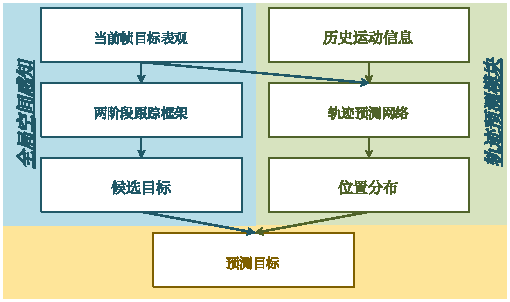
\includegraphics[width=0.8\textwidth]{Img/globally/Arch7.pdf}
    \caption{我们基于全局时空感知(GSTP)的跟踪系统的架构。}
\end{figure}

视频目标跟踪 \cite{Leang2018OnlineFO, Wang2019VisualOT, Zhang2018UsingFL} 是计算机视觉领域中一个具有挑战性的任务,旨在建立连续视频序列中待跟踪目标的位置关系。
流行的孪生网络跟踪器 \cite{SiamFC, SiamRPN, Wang2018SiamMask} 通常基于局部搜索机制:在以前一帧的目标位置为中心的小邻域内搜索目标,从而中确定其在当前帧中的位置。
如果目标仅在两个相邻帧之间具有较小的位移,则此机制可发挥正常作用。该局部搜索机制的另外一个好处是可以避免来自背景中近似物体的干扰。

然而,局部搜索机制存在一些缺点:

\begin{itemize}
\item 首先,如果由于挑战性的照明变化、运动模糊等原因导致先前帧中目标位置的预测偏离了预期,则在当前帧生成的搜索区域可能会无法覆盖真实目标的位置,从而导致不可逆的累积误差,在后续帧彻底跟丢目标。
\item 其次,基于局部搜索机制的跟踪器很难满足长期跟踪的需求 \cite{kalal2011tracking, hong2015multi}。
在长期跟踪情况下,目标经常退出并重新进入画面。
当目标离开画面或重新进入画面时,跟踪器无法设置正确的搜索区域,一旦由于搜索区域设置错误而没有覆盖真实目标的位置,则跟踪器通常无法检索目标。
\end{itemize}

受 Faster RCNN 的两阶段检测框架 \cite{ren2015faster} 的启发,本章提出了一种基于全局感知机制的两阶段孪生网络跟踪器。
在跟踪过程中,所提出的跟踪器始终能够感知整个图像中的目标。
因此,即使跟踪器由于具有挑战性的目标表观变化而犯了一个错误,一旦目标的表观恢复正常,跟踪器便可以及时检索目标。尤其是在长期跟踪中目标离开画面的情况下,当目标从任何位置重新进入画面时,跟踪器便可以继续工作。

所提出的全局感知机制的另一个优势是,跟踪器可以结合 RoI Align \cite{He2018MaskR} 操作,利用更深的网络进行特征学习,而这对于流行的基于局部搜索机制的 SiamFC \cite{SiamFC} 和 SiamRPN \cite{SiamRPN} 跟踪器来说是难以实现的,因为其网络结构中的填充操作将破坏严格的平移不变性 \cite{SiamRPN++},因此尽可以使用浅层神经网络进行特征学习。具体来说,在本章提出的跟踪器中,我们将整个模板图像和搜索图像送入相同的主干网络以提取特征,然后根据初始帧的真实标注信息使用 RoI Align 操作从模板特征中提取目标特征。通过逐通道互相关操作使目标特征和搜索图像特征进行融合,以获得融合特征图,该融合特征图被送入后续的跟踪模块以得到最终的跟踪位置。由于该跟踪框架对平移不变性没有任何限制,因此可以使用具有较强特征提取能力的 ResNet \cite{he2016deep} 作为主干网络来提高跟踪器对前景目标与背景噪声之间的判别性。

除了上述全局空间感知机制外,本章还提出了一种轨迹预测模型来减轻近似物体的干扰,以解决端到端训练的孪生网络跟踪器难以区分表观近似目标的问题。与简单设计的手工策略 \cite{SiamFC, SiamRPN} 不同,本章提出的基于卷积神经网络的轨迹预测模型经过端到端训练,可以使用目标的历史轨迹信息和当前帧中的目标表观信息来预测目标在当前帧中的位置分布。
具体来说,目标的运动模式是在训练阶段从大规模轨迹数据集自动学习的,而不是基于手工制作的特征或规则 \cite{iswanto2017visual};在测试阶段,我们可以使用任意数量的历史帧位置信息,而不是仅基于上一帧的目标位置进行预测。

综上所述,本章做出以下三个主要贡献。
\begin{itemize}
\item 基于全局感知机制,我们引入了一个两步跟踪管道,该管道使用非常深的网络来减少累积误差并提高鲁棒性。
\item 提出了一种新颖的统一的端到端卷积神经网络的轨迹预测结构,利用历史轨迹信息和当前帧的出现信息来预测目标位置分布。
\item 我们在 GOT-10k \cite{GOT-10k} 和UAV20L \cite{mueller2016benchmark} 长期跟踪数据库上优秀的性能证明了我们提出的基于全局时空知觉的跟踪系统(GSTP)的有效性。
\end{itemize}

\iffalse
\section{相关工作之目标跟踪中的运动模型}
在目标跟踪中,运动模型是一个重要的环节。运动模型在目标跟踪中的作用是依据上一帧目标的位置预测在当前帧目标可能出现的区域。在基于孪生网络的目标跟踪中,通常采用静止运动模型。一些工作采用匀加速度运动模型对物体的运动进行建模也带来了性能提升。
\fi

\begin{figure}[t]
    \centering
    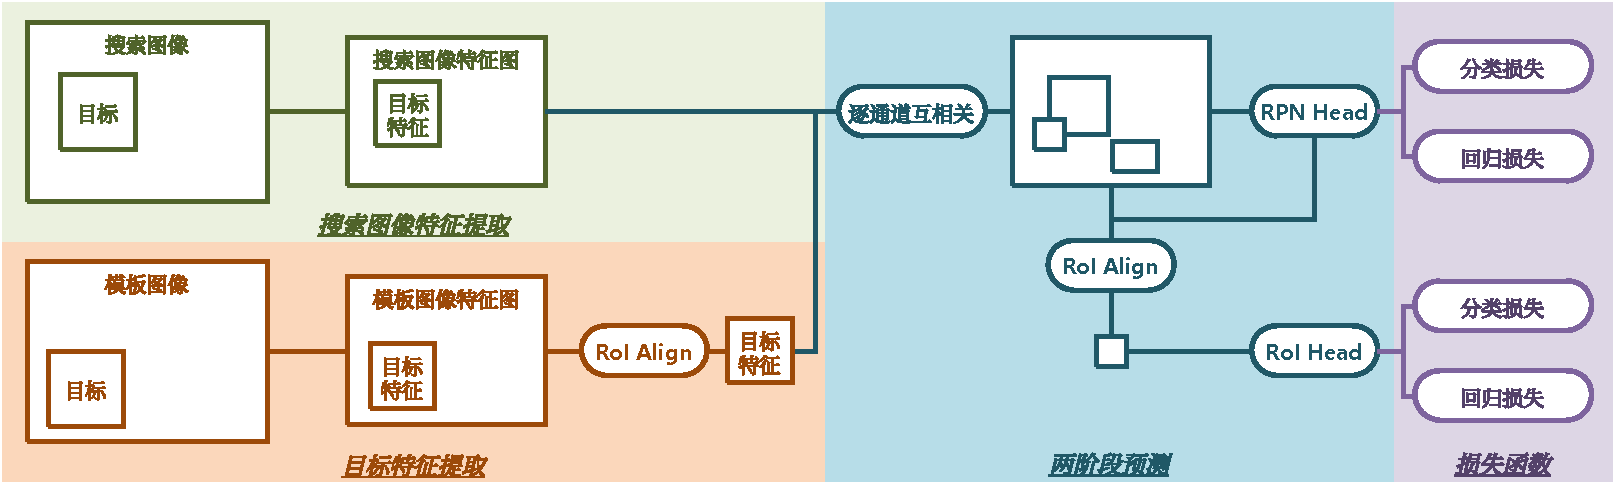
\includegraphics[width=1.0\textwidth]{Img/globally/SiamRCNN.pdf}
    \caption{本章所提算法的网络结构示意图。}
    \label{fig:siamrcnn}
\end{figure}

\section{空间信息增强的视频目标跟踪算法}

\iffalse
\begin{figure*}
    \centering
    \includegraphics[width=12cm]{images/NetworkStructure1.pdf}
    \caption{The proposed tracking framework.}
    \label{fig:network}
\end{figure*}
\fi

\iffalse
\begin{figure*}
    \centering
    \includegraphics[width=12cm]{images/MotionModel.pdf}
    \caption{The effect of the motion model. SiamRCNN detects the real target (in green box) and the distractor (in red box). The motion model predicts the position distribution measuring the likelihood that the target is located at each spatial location. The motion model eliminates the distractor and preserves the real target.}
    \label{fig:motion_model}
\end{figure*}
\fi

在本章中,我们采用如下步骤进行视频目标跟踪任务:首先基于全局感知机制提取候选目标区域,然后使用轨迹预测模块消除近似物体的干扰。通过采用该跟踪流程,我们可以通过设计更精确的候选目标提取模块和更鲁棒的的轨迹预测模型共同提升孪生网络的目标跟踪性能,尤其是长期目标跟踪性能。

总体而言,本章提出了空间信息增强的全局感知系统具有如下贡献:
\begin{itemize}
\item 我们使用整个图像而不是小的图像块作为跟踪器的输入,以为跟踪器提供更丰富的全局空间信息。
\item 为了更好地感知全局空间信息,本章提出了一个两阶段跟踪框架,该框架能够检测在视觉表观上类似于真实目标的候选目标区域。
\item 为了消除候选目标区域中近似物体的干扰,本章提出了一个轨迹预测模块,该模块能够通过预测目标在当前帧的位置分布以排除近似物体,获得最终的跟踪结果。
\end{itemize}

\iffalse
Most state-of-the-art trackers adopt a one-stage framework, which performs classification and bounding box regression only once based on features obtained by cross-correlation.
In the field of object detection, the performance of two-stage detectors is usually better than that of one-stage detectors.
Inspired by this, we design our tracker as a two-stage network.
The RPN stage rapidly filters out most background samples, and the RoI head adopts a fixed foreground-to-background ratio to maintain a manageable balance between foreground and background.
In addition, two steps of regressions achieve accurate localization even for objects with extreme shapes.
\fi

\begin{figure}[t]
\centering
    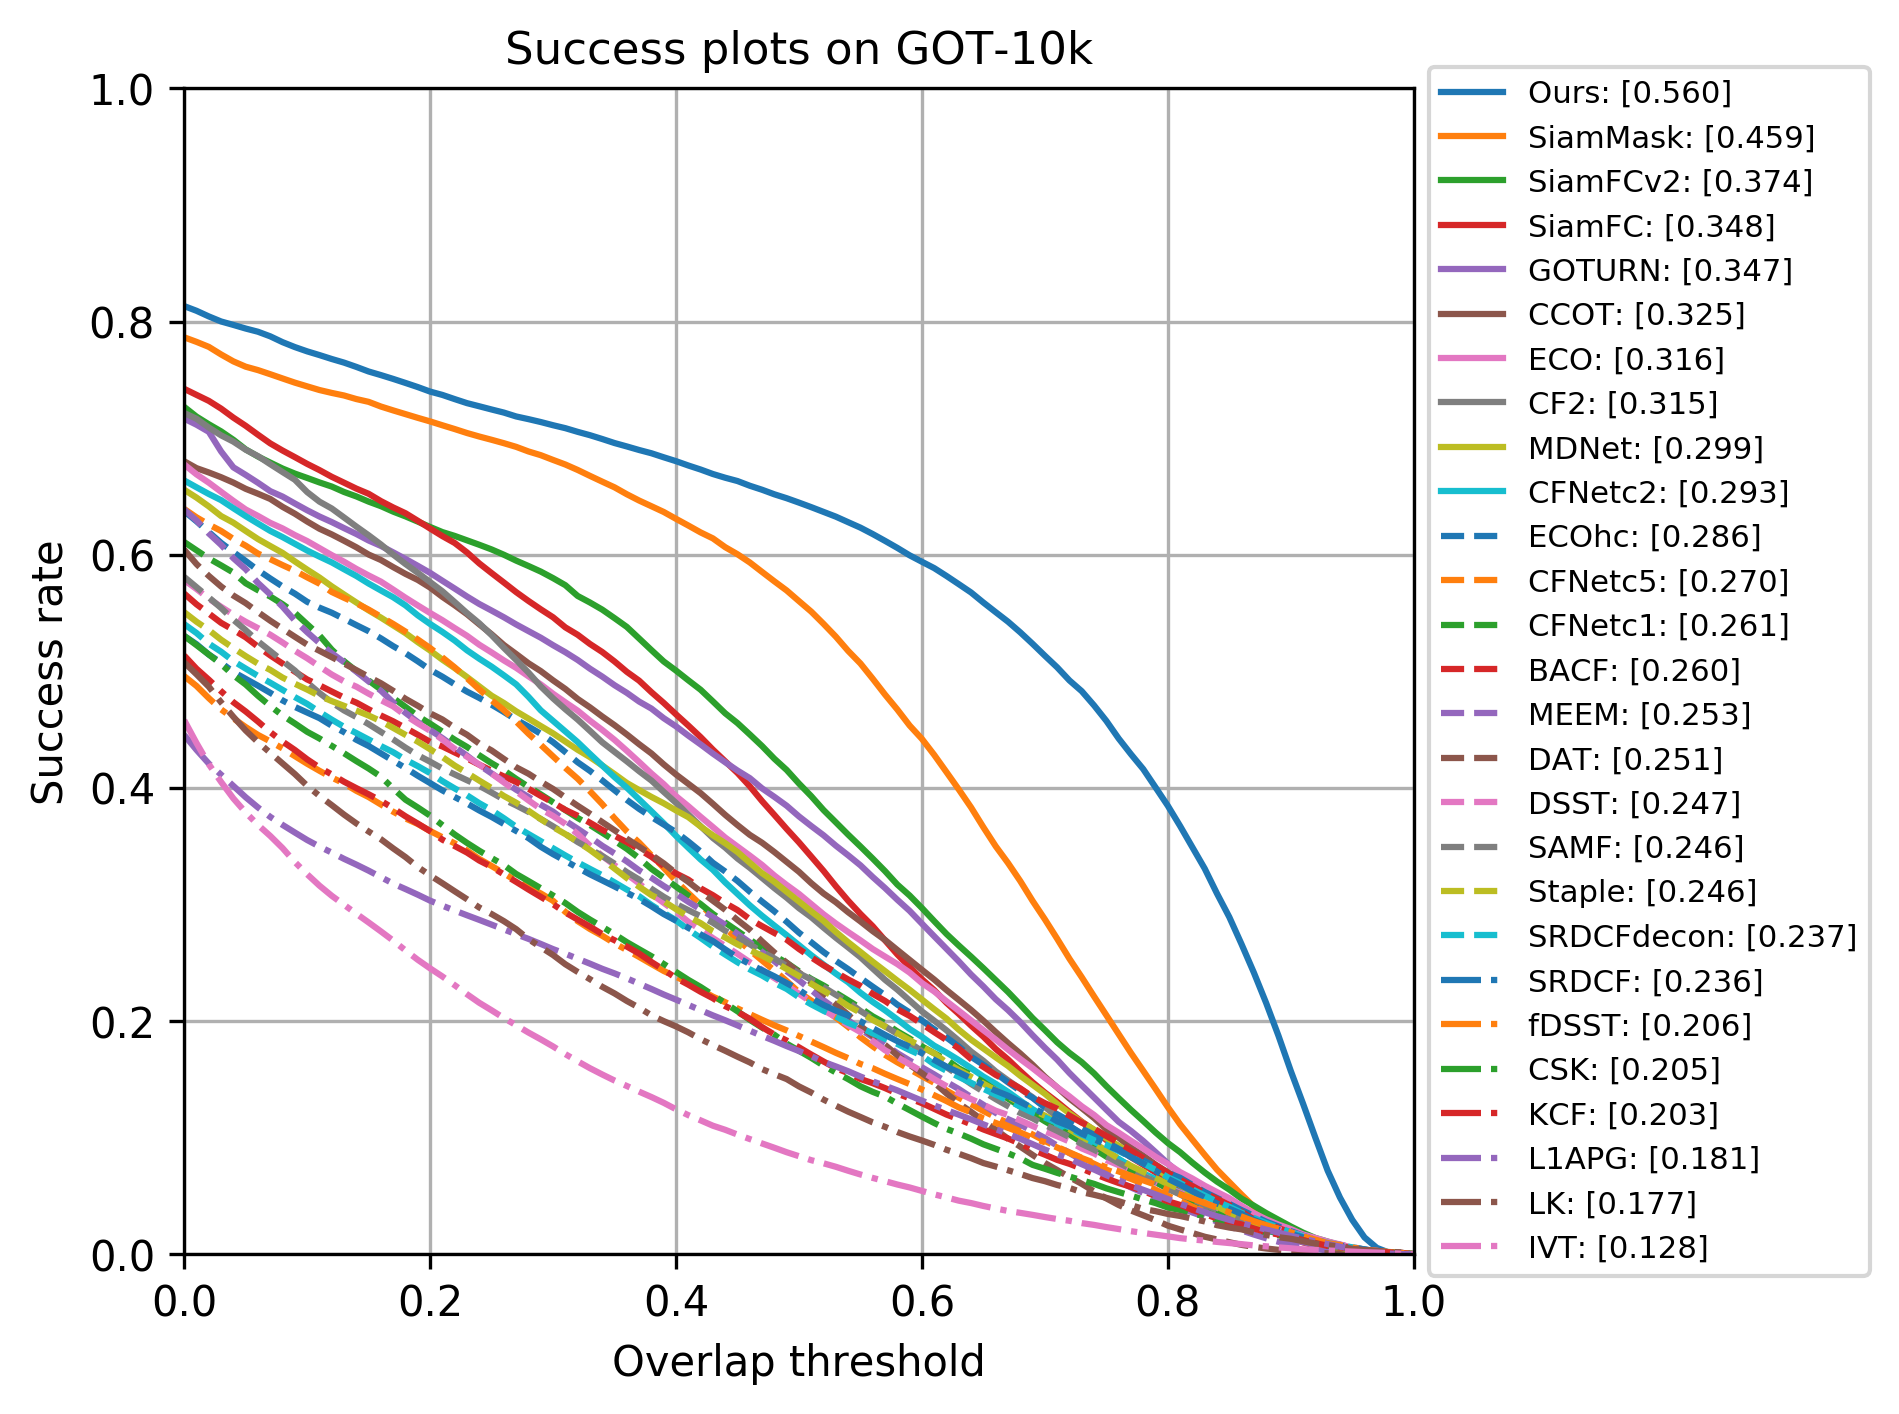
\includegraphics[width=0.75\textwidth]{Img/globally/success_plot.png}
    \caption{GOT-10k 的总体性能,按平均重叠(AO)得分进行排名。}
\end{figure}

\subsection{两阶段跟踪框架}

我们基于流行的目标检测架构 Faster RCNN \cite{ren2015faster} 来构建跟踪框架。尽管利用目标检测模块和孪生网络进行视频目标跟踪并非在本章中首次提出,但本章提出的视频目标跟踪算法与类似视频目标跟踪方法 \cite{SiamRPN, Wang2018SiamMask, danelljan2019atom, voigtlaender2019siam} 相比具有优势。与 SiamRPN \cite{SiamRPN}相比,SiamRPN 的网络输入始终是目标位于中心的图像块,而本章提出的跟踪算法的输入是整个图像,这意味着目标可能出现在图像中的任何空间位置。这防止了网络学习到偏向中心位置的错误先验,从而打破了空间不变性约束 \cite{SiamRPN++} 对于网络体系结构设计的限制。因此,可以采用非常深的卷积神经网络(例如ResNet50 \cite{he2016deep})用于跟踪算法的特征提取器。有关空间不变性玉树和中心位置偏差的详细说明,请参考 \cite{SiamRPN++}。
%because the input of the network is the entire image, instead of the image patch centered on the target, the target will appear in any poisition in the image, so we do not need the network has strict spatial invariance restriction \cite{SiamRPN++}, so we can use a deeper feature extractor, i.e., resnet50. 
与 SiamRPN \cite{SiamRPN} 和 SiamMask \cite{Wang2018SiamMask} 相比,本章提出的跟踪算法采用两阶段体系结构。第二阶段(RoI head \cite{ren2015faster})可以更有效地区分前景和背景。
与 SiamMask \cite{Wang2018SiamMask} 和 ATOM \cite{danelljan2019atom} 相比,本章的跟踪器可以在整个图像中搜索目标,从而在由于遮挡、运动模糊等原因导致跟踪结果出错后,仍可在目标表观恢复正常时重新跟踪目标。
与 Siam R-CNN \cite{voigtlaender2019siam} 相比,Siam R-CNN 的特征提取网络和 RPN 的网络参数是冻结的,未针对视频目标跟踪任务进行端到端训练,而本章提出的跟踪器中,特征提取网络可以生成特定于目标的特征,并且可以端到端地训练整个网络。在视频目标跟踪中,一个视频中的前景目标可能是另一个视频中的背景噪声。因此,本章跟踪器中的 RPN 模块生成的候选目标区域可以更好地满足通用目标跟踪的需求。

\begin{figure}[t]
\begin{minipage}{0.48\linewidth}
  \centering
  \centerline{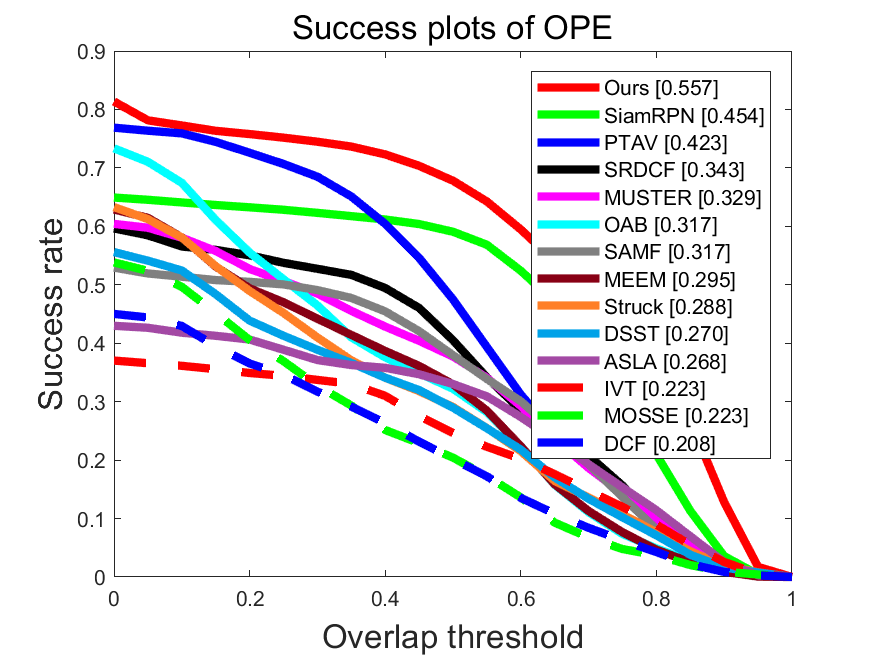
\includegraphics[width=1.0\textwidth]{Img/globally/UAV20L/quality_plot_overlap_OPE_AUC.png}}
\end{minipage}
\hfill
\begin{minipage}{0.48\linewidth}
  \centering
  \centerline{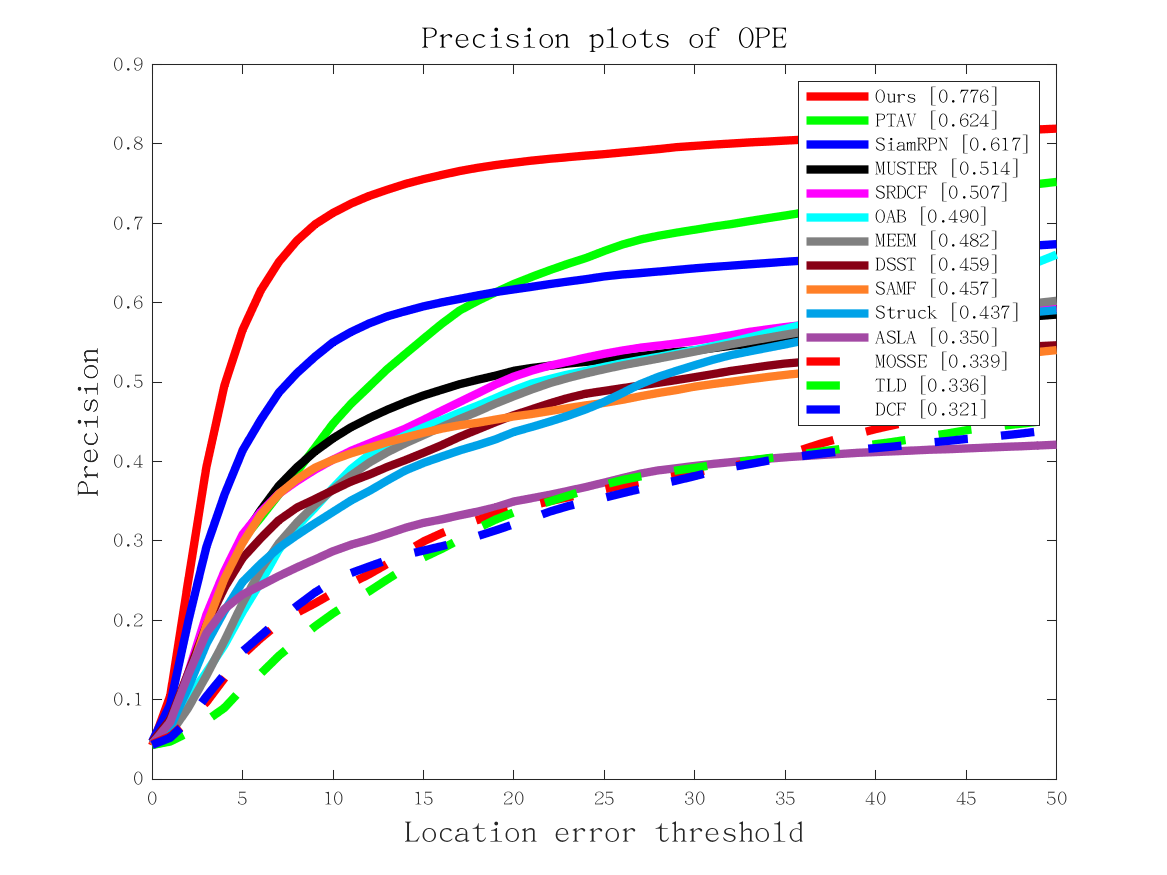
\includegraphics[width=1.0\textwidth]{Img/globally/UAV20L/quality_plot_error_OPE_threshold.png}}
\end{minipage}
\caption{UAV20L 数据集上的成功图和精度图。}
\label{fig:globally_uav20l}
\end{figure}

%(The backbone and RPN are frozen and only the redetection head (after concatenation) is trained for tracking) they fixed the parameters in the backbone and the RPN. Only the second stage is used for target spercific tracking, which is not good for "generatic" object tracking: because some objects are foreground in some cases and background in others. Instead, our tracker use the correlation before RPN, the "target" which is good for general object tracking. The architecture of our tracking component is described as follows:

%The first component of our tracking framework (i.e., SiamRCNN) is a two-stage tracker (Fig. \ref{fig:siamrcnn}) used to detect object regions that are visually similar to the given first-frame template object.
%Specifically, the tracking component consists of four modules: (1) feature extraction module, (2) feature fusion module, (3) RPN head module, and (4) RoI head module.

%The transplant from a detection task to a tracking task using faster RCNN is straightforward and easy to implement.
%, which is another advantage of our tracking module. 
为了描述本章提出的跟踪框架,我们首先简要回顾一下 Faster RCNN。该目标检测网络包括一个特征提取器,其后是两个检测模块:RPN 头和 RoI 头。
特征提取器 $\phi_{1}$ 是 ResNet50 的变体。第一阶段使用区域生成网络(RPN)在特征提取网络的最后一个特征图上执行滑动窗口操作,在判断每个空间位置是否存在目标的同时,预测这些目标的边界框。
在第二阶段(即 RoI head)中,区域生成网络生成的每个候选区域,利用 RoI Align \cite{He2018MaskR} 操作提取尺度相同的深度特征
使用分类层将每个候选区域(region of interest,ROI)分类为特定类别,并使用回归层对边界框位置进行进一步微调。请参阅 \cite{ren2015faster} 了解更多详细信息。

对于目标跟踪任务,特征提取器 $\phi_{1}$ 有两个输入:模板图像 $z$ 和搜索图像 $x$。根据孪生架构的设计,两个输入共享相同的网络参数以提取特征。
在生成模板特征 $f_{z} = \phi_{1}(z)$ 和搜索特征 $f_{x} = \phi_{1}(x)$ 之后,利用 RoI Align 操作 \cite{He2018MaskR},根据目标的真实标注框,模板特征中裁剪得到目标特征 $f_{obj} \in \mathbb{R}^{1024 \times 7 \times 7}$:
\begin{equation}
    f_{obj} = \mathcal{R}(b_{obj}, f_{z}),
\end{equation}
其中 $\mathcal{R}$ 表示 RoI Align 运算符,而 $b_{obj}$ 是目标的真实边界框。
接下来,通过逐通道互相关 \cite{SiamRPN++} 操作融合搜索特征和目标特征:
\begin{equation}
    f_{corr} = f_{obj} * f_{x},
\end{equation}
其中 $f_{corr}$ 是融合特征,$*$ 是逐通道互相关算子。
%The use of RPN (region proposal network) is ...
然后将 $f_{corr}$ 发送到 RPN head 以生成候选目标 $B=\{b^{i}_{roi}\}^{i=1:N}$。
\iffalse
There are two inputs to the feature extraction module: the template image $z$ and the search image $x$. According to the design of the siamese architecture, the two inputs share the same network parameters to extract features.
The network structure of the feature extraction module is a variant of ResNet50, which is pretrained on the 1000-class ImageNet classification set. Features of the input images are extracted from the final convolution layer of the 4-th stage. The obtained template features $f_{z} = \phi(z)$ and search features $f_{x} = \phi(x)$ with channel dimension 1024 and stride 16 are sent to the subsequent feature fusion module.

In the feature fusion module, object features $f_{obj}$ are obtained by the RoI Align operation from the template features according to the ground truth of the target. The search features and the object features are merged via the depth-wise cross-correlation:
\begin{equation}
    f_{obj} = \mathcal{R}(b_{obj}, f_{z})
\end{equation}
where $\mathcal{R}$ represents the RoIAlign, $\odot$ represents the element-wise multiplication, $b$ represents an RoI in candidate proposals and $\mathcal{X}$ represents the fused feature of $b$.
\begin{equation}
    f_{corr} = f_{obj} * f_{x}.
\end{equation}
Two 1 $\times$ 1 convolutions with channel dimension 1024 are added on top of the correlation layer to obtain the fusion feature.

The RPN head includes two sibling 1 $\times$ 1 convolutional layers -- a classification layer with channel dimension 2$k$, and a regression layer with channel dimension 4$k$, where $k$ is the number of maximum possible proposals for each location. The RPN head takes the fusion feature as input and simultaneously regress region bounds and objectness scores for each anchor.
\fi
%The RoI head is run for each region proposed by the RPN by performing RoI Align \cite{He2018MaskR} to extract deep features from this proposed region.
在第二阶段,对融合特征 $f_{corr}$ 执行 RoI Align 操作,为每个 RoI 生成一个小特征图,其通道尺寸为 2048,空间分辨率固定为 7 $\times$ 7:
\begin{equation}
    f_{roi}^{i} = \mathcal{R}(b_{roi}^{i}, f_{corr}),
\end{equation}
其中 $b_{roi}^{i}$ 是候选区域 $i$ 的边界框。
最后,每个 RoI 被分类为前景或背景。在测试期间,我们选择排名靠前的 $K$ 的 RoI 作为候选目标,这些目标将在轨迹预测模块中进行后处理。

\iffalse
The RoI Aligned features are fed into the global average pooling layer followed by two sibling output layers: one that produces softmax probability estimates over two classes (foreground or background) and another layer that outputs four real-valued numbers for the foreground class. These four values encode the refined bounding-box position for the RoI.
The loss of SiamRCNN is:
$$Loss = L_{cls}^{rpn} + L_{cls}^{roi} + \lambda (L_{reg}^{rpn}+L_{reg}^{roi}),$$
where $\lambda$ is hyper-parameter to balance the classification loss and the regression loss. $L_{cls}^{*}$
is the cross entropy loss and $L_{reg}^{*}$ is the standard smooth $L1$ loss for regression.
\fi

\begin{table}[t]
\centering
\caption{本章提出的算法在 GOT-10k 测试集上,不同组件的性能。}
\begin{tabular}{c c c c c}
\bottomrule
ROI head & Motion model & $AO$ & $SR_{0.50}$ & $SR_{0.75}$ \\ 
\hline
          &           & 0.410 & 0.486 & 0.162 \\
\checkmark&           & 0.521 & 0.595 & 0.440 \\
\checkmark&\checkmark & 0.560 & 0.645 & 0.457 \\
\bottomrule
\label{table:globally_ablition}
\end{tabular}
\end{table}

\subsection{轨迹预测模块}
使用前文提出的的跟踪框架提取到与给定的第一帧模板目标在视觉表观上相似的候选目标区域后,我们利用轨迹预测模块消除近似物体的干扰并获得最终的跟踪结果。
轨迹预测模块以端到端的方式,使用目标的历史轨迹信息和当前帧的表观信息学习目标位置分布,该目标位置分布是一个二维热图,用于度量目标位于每个空间位置的可能性,我们根据该目标位置分布信息重新评估每个候选目标。

\begin{table}[t]
\centering
\caption{将本章提出的方法与其他视频目标跟踪方法在 GOT-10k 测试集上的跟踪结果进行比较。跟踪器按其平均重叠(AO)分数排名。}
\begin{tabular}{l l l l}
\bottomrule
Method   &  $AO$   &  $SR_{0.50}$ & $SR_{0.75}$  \\
\hline
Ours &  $\textbf{0.560}^\textbf{1}$ & $\textbf{0.645}^\textbf{1}$  & $\textbf{0.457}^\textbf{1}$  \\
SiamMask &  0.459&  0.560 &0.205 \\
SiamFCv2 &  0.374&  0.404 &0.144 \\
SiamFC   &  0.348&  0.353 &0.098 \\
GOTURN	 &  0.347&  0.375 &0.124 \\
CCOT	 &  0.325&  0.328 &0.107 \\
ECO	     &  0.316&  0.309 &0.111 \\
CF2	     &  0.315&  0.297 &0.088 \\
MDNet	 &  0.299&  0.303 &0.099 \\
CFNetc2	 &  0.293&  0.265 &0.087 \\
ECOhc	 &  0.286&  0.276 &0.096 \\
\bottomrule
\end{tabular}
\label{table:got}
\end{table}

令 $H_{t}^{k} = \{h_{t-i}\}_{i=1:k}$ 表示历史轨迹信息,其中 $t$ 是当前帧的索引,$k$ 是历史长度,并且 $h_{j} = \{x_{j}, y_{j}\}$ 是一个二维坐标,表示目标在帧 $j$ 中的位置。
受姿态估计任务的启发,我们将 $h_{j}$ 表示为二维热图 $m_{j} \in \mathbb R^{h \times w}$,其中二维高斯顶点位于目标位置 $(x_{j}, y_{j})$。
为了对目标的轨迹信息进行建模,我们根据时间顺序将生成的 $k$ 热图进行串接,以获得通道维度为 $k$ 的轨迹张量 $\mathcal{M} \in \mathbb{R}^{k \times h \times w}$:
\begin{equation}
    \mathcal{M}_{t}^{k} = \mathcal{C}(m_{t-k}, m_{t-k+1}, ..., m_{t-1}),
\end{equation}
其中 $\mathcal{C}(\cdot)$ 表示串联操作。

本章提出的轨迹预测模块不仅利用历史轨迹信息进行预测,同时页考虑当前帧的表观信息。
为此,将当前帧 $\mathcal{I} \in \mathbb{R}^{3 \times h \times w}$ 的 RGB 图像与轨迹张量串接起来,以获得增强的轨迹张量 $\mathcal{N} \in \mathbb{R}^{(3+k) \times h \times w}$,通道尺寸为 $(3+k)$:
\begin{equation}
    \mathcal{N}_{t}^{k} = \mathcal{C}(\mathcal{I}_{t}, \mathcal{M}_{t}^{k}).
\end{equation}
假设 $\phi_{2}$ 是基于卷积神经网络的轨迹预测模型,则 $\phi_{2}$ 的输出计算如下:
\begin{equation}
    \mathcal{O}_{t}^{k} = \phi_{2}(\mathcal{N}_{t}^{k}),
\end{equation}
其中 $\mathcal{O}_{t}^{k} \in \mathbb{R}^{h \times w}$ 是二维热图,它反映了目标在 $t$ 帧中的位置分布。

本章提出的运动模型 $\phi_{2}$ 的网络与姿势估计网络 HRNet \cite{sun2019deep} 相同。
\iffalse
The main reason why the pose estimation network can be used to design the motion model is that the output of the pose estimation network is the position distribution of joint points, and the output of the motion model is the position distribution of the target. This means that there is a great deal of commonality between the two tasks. In order to use HRNet for trajectory estimation, we need to change the input and output of HRNet and keep the network structure unchanged.

During tracking the $i$-th frame, we utilize the position information of the previous $K$ frames as the input to the network.
Specifically, for a historical frame, a heat map is generated by applying 2D Gaussian with stand deviation of 3 pixels centered on the target position in that frame.
The generated $K$ heatmaps are concatenated according to the time order to obtain the \textbf{trajectory tensor} with channel dimension $K$.
Our motion model not only utilizes the historical trajectory information for prediction, but also considers the appearance information of the current frame.
To achieve this, the RGB image of the current frame and the trajectory tensor are concatenated to obtain the tensor with channel dimension $(3+K)$. This tensor is sent to the network, and the output of the network is a heatmap reflecting the position distribution of the target in the current frame. The loss function, defined as the mean squared error, is applied for comparing the predicted heatmap and the groundtruth heatmap. The groundtruth heatmap is generated by applying 2D Gaussian with standard deviation of 3 pixels centered on the target position in the current frame. The network structure of our motion model is the same as HRNet. 
\fi
这里提供简要说明。HRNet 的第一阶段是高分辨率子网。在此基础上依次添加从高分辨率到低分辨率的子网,以形成更多的阶段。多分辨率子网之间并行连接。通过在整个网络中重复地在并行多分辨率子网中交换信息来进行多尺度融合。我们利用 HRNet 的高分辨率输出来表示目标的位置分布。有关网络结构的详细信息,请参考 \cite{sun2019deep}。

\begin{table}[t]
\centering
\caption{从 GOT-10k 验证集中收集的具有不同属性子集的性能。}
\begin{tabular}{|c|c|c|c|c|c|c|}
\hline
\multirow{2}{*}{属性} &
\multicolumn{2}{c|}{SiamFC} & \multicolumn{2}{c|}{SiamMask} &\multicolumn{2}{c|}{本章方法} \\
\cline{2-7} & $AO$ & $SR_{0.5}$ & $AO$ & $SR_{0.5}$ & $AO$ & $SR_{0.5}$ \\
\hline
快速运动 & 0.472 & 0.538 & 0.526 & 0.608 & 0.639 & 0.715 \\
\hline
遮挡 & 0.411 & 0.447 & 0.494 & 0.559 & 0.585 & 0.659 \\
\hline
图像边界切割 & 0.505 & 0.545 & 0.595 & 0.701 & 0.738 & 0.837 \\
\hline
长视频 & 0.557 & 0.655 & 0.643 & 0.779 & 0.721 & 0.807 \\
\hline
\end{tabular}
\label{table:attribute}
\end{table}

\section{实验结果与分析}

\subsection{实验设置}

\begin{figure*}[t!]
\begin{center}
	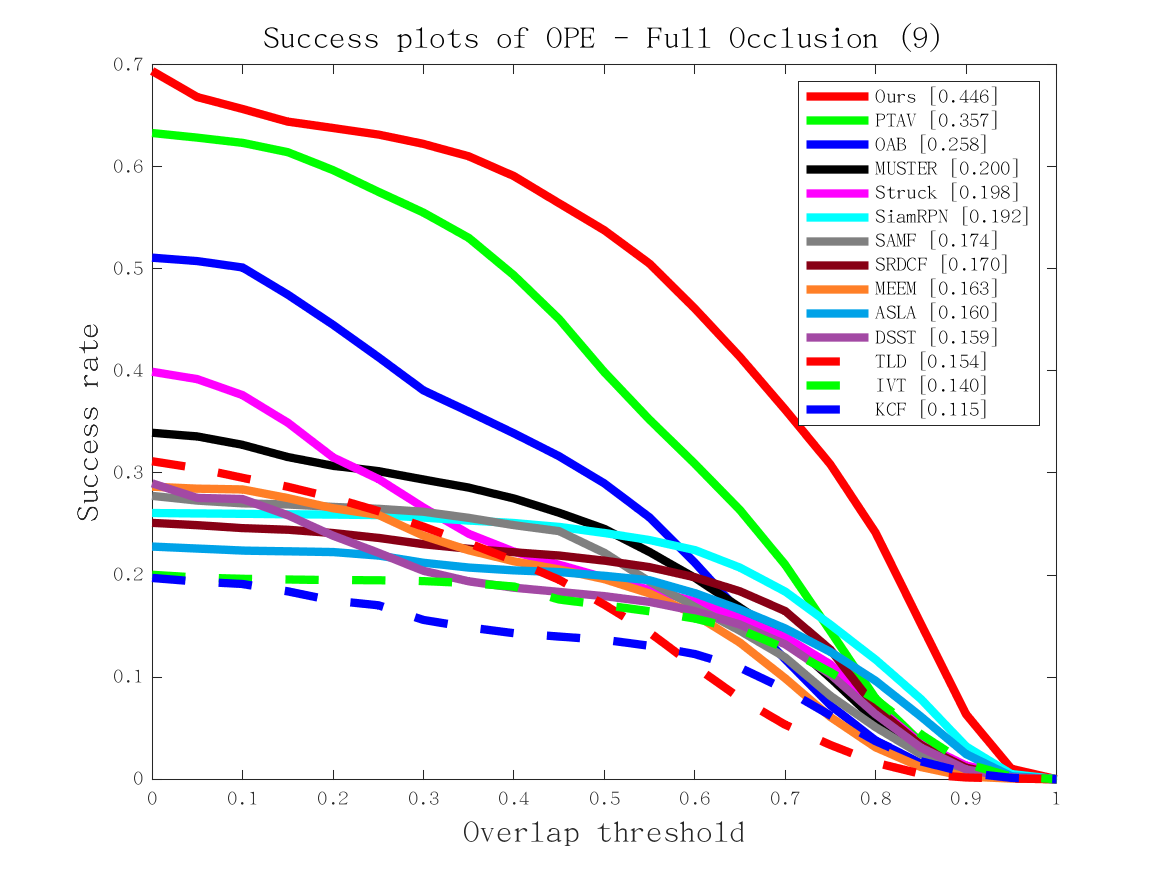
\includegraphics[width=0.48\textwidth]{Img/globally/UAV20L/FOC_overlap_OPE_AUC.png}
	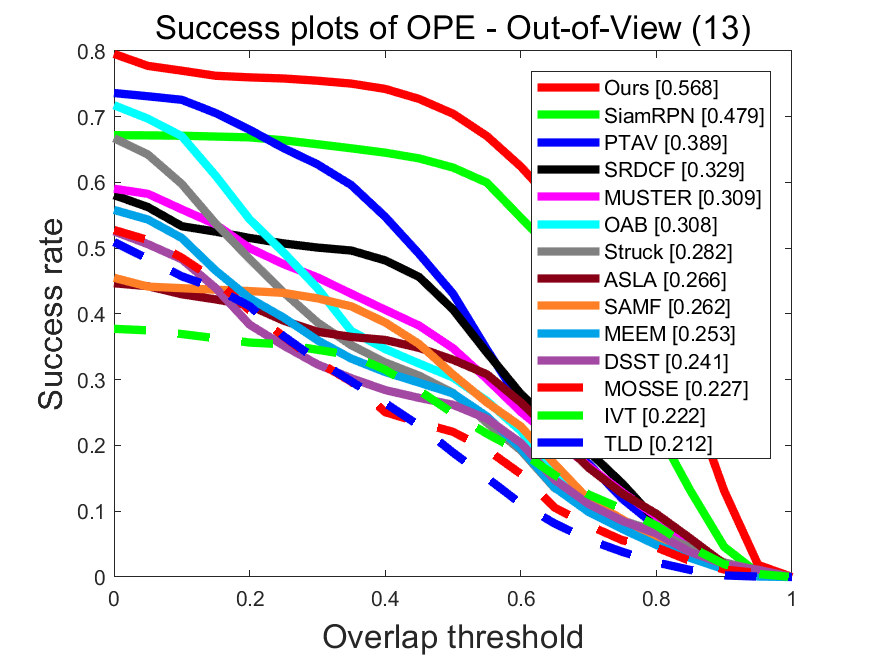
\includegraphics[width=0.48\textwidth]{Img/globally/UAV20L/OV_overlap_OPE_AUC.png}
	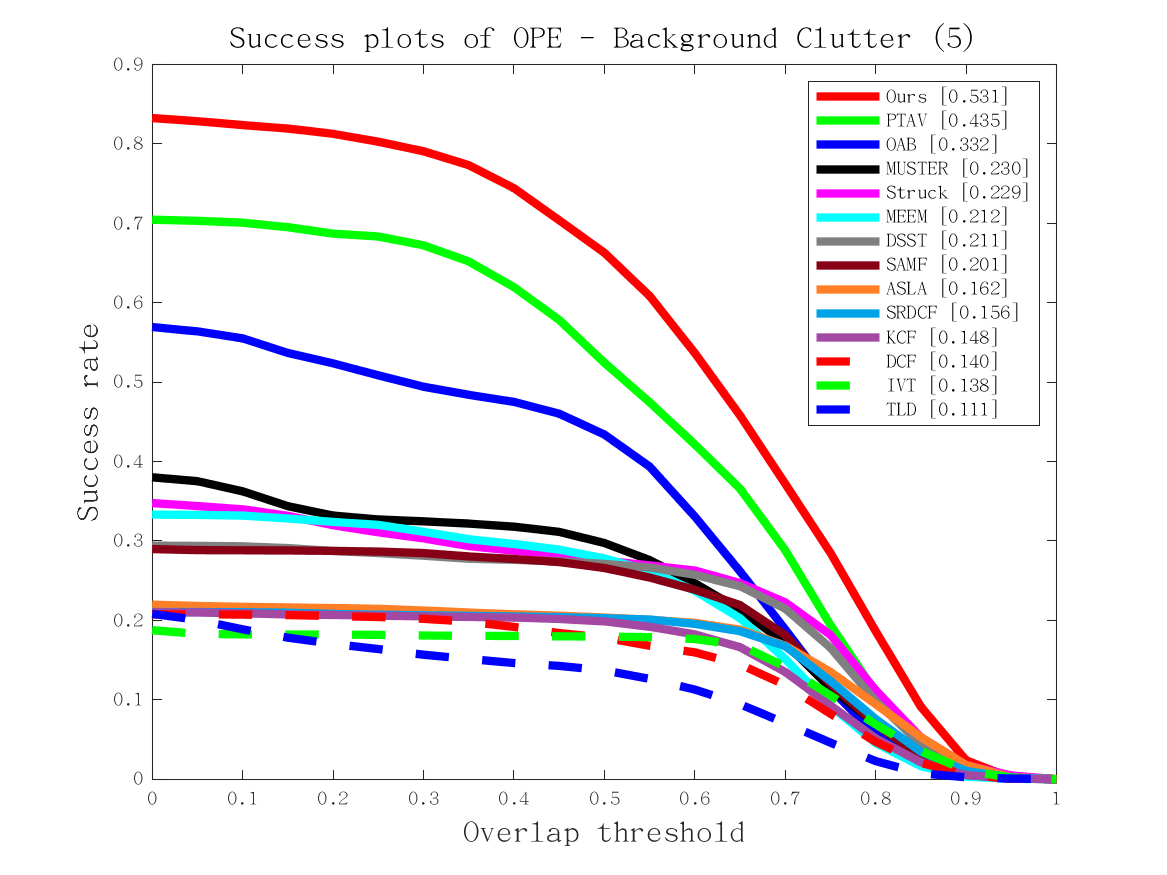
\includegraphics[width=0.48\textwidth]{Img/globally/UAV20L/BC_overlap_OPE_AUC.png}
	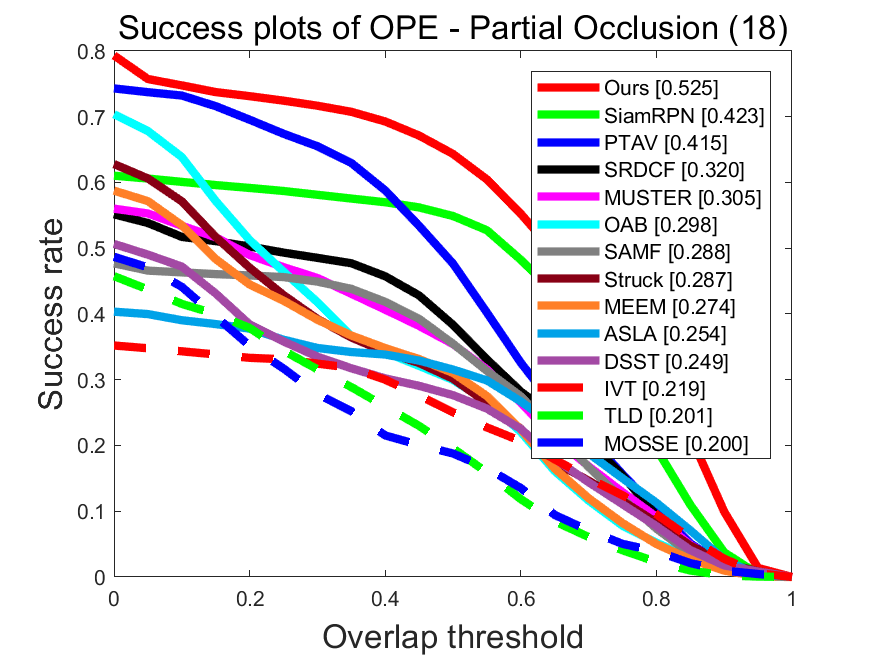
\includegraphics[width=0.48\textwidth]{Img/globally/UAV20L/POC_overlap_OPE_AUC.png}
	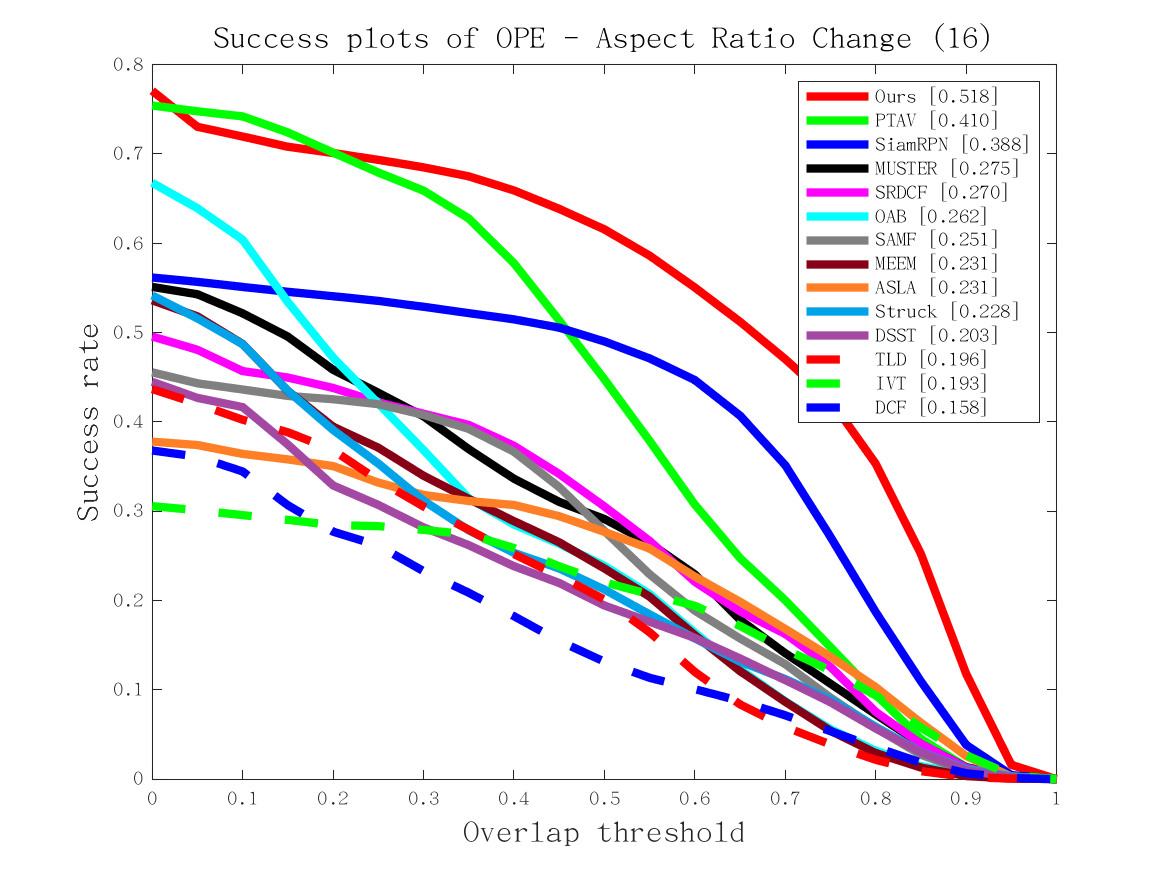
\includegraphics[width=0.48\textwidth]{Img/globally/UAV20L/ARC_overlap_OPE_AUC.png}
	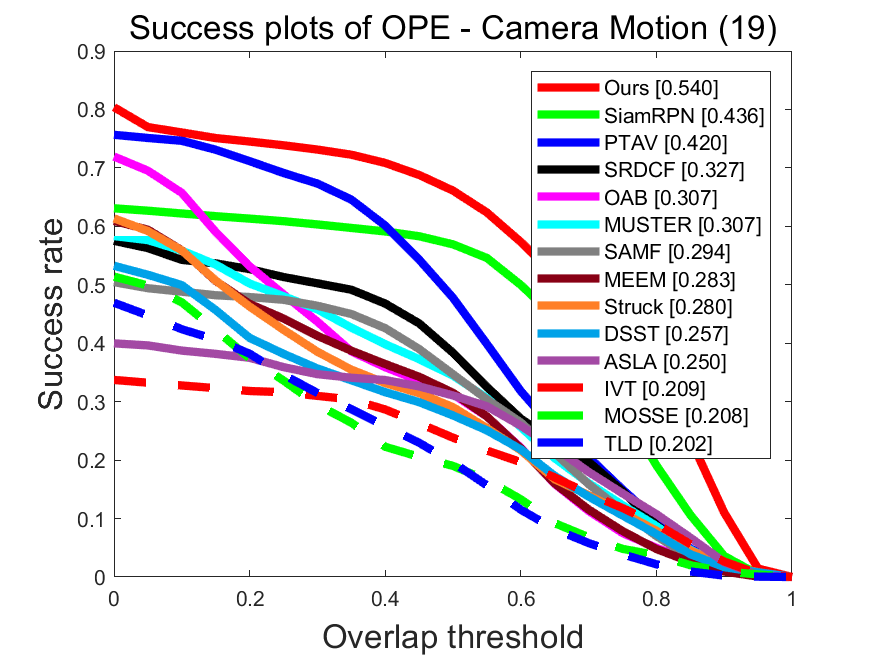
\includegraphics[width=0.48\textwidth]{Img/globally/UAV20L/CM_overlap_OPE_AUC.png}
\end{center}
   \caption{在 UAV20L 上成功绘制带有属性的图 1。在彩色显示屏上观看效果最佳。}
\label{fig:globally_uav20l_1}
\end{figure*}

\textbf{网络架构设计}:本章提出的空间信息增强的孪生视频目标跟踪网络主要有三个子网络组成,分别是用于共享特征提取的主干网络、用于生成特定目标特征的特征调制子网络以及用于边框微调的区域细化子网络。它们的网络结构如图 \ref{fig:siamrcnn} 所示,主干网络基于 ResNet-50 设计,可以为模板图像和搜索区域图像提取深度特征,以提升特征表示能力。

\textbf{训练数据}:为了提高特征表示的泛化能力和判别能力,同时避免在稀缺的跟踪数据上过拟合,离线训练过程在大规模单目标视频跟踪数据库 GOT-10k \cite{GOT-10k} 的训练数据集中训练网络参数。GOT-10k 数据集具有超过 10000 个真实运动目标的视频片段和超过 150 万个手动标记的边界框,包括 563 类真实运动目标和 87 类运动模式。
我们执行多尺度训练:目标大小从 $64 \times 64$ 至 $256 \times 256$ 不等。图像大小在跟踪过程中保持不变。

\textbf{优化器参数设定}:本章使用动量为 0.9 的随机梯度下降(stochastic gradient descent,SGD)优化器从在 ImageNet 上预训练的网络参数开始训练,并将权值衰减参数设置为 $10^{-4}$。学习率从 $10^{-2}$ 指数衰减到 $10^{-4}$。该模型经过 27000 次迭代训练,每个批次大小为 2 个样本对。

本章提出的轨迹预测模块也利用 GOT-10k 训练集进行训练。训练采用的优化器为 Adam 优化器 \cite{kingma2014adam}。初始学习率设置为 $10^{-3}$,并在第 170 轮和 200 轮迭代时分别降至 $10^{-4}$ 和 $10^{-5}$。训练过程在 210 轮迭代后终止。

本章所提出的时间信息增强的孪生网络跟踪器使用 Pytorch 在 Python 中实现,所有实验在装配有 Intel(R) Xeon(R) CPU E5-2630 v4 @ 2.20GHz 和 NVIDIA TITAN 1080Ti GPU 的工作站上执行。

\subsection{对 GOT-10k 数据集的评估}
在本节中,我们在 GOT-10k \cite{GOT-10k} 数据集上评估所提出的跟踪算法。
GOT-10k 的评价指标包括平均重叠(AO)和成功率(SR)。AO 表示所有真实边界框和预测边界框之间重叠的平均值,而 SR 表示重叠超过 0.5/0.75 的成功进行跟踪的帧占总帧数的百分比。

\textbf{对比实验}
为了分析本章提出的两阶段跟踪框架和轨迹预测模块的有效性,我们训练了两个跟踪网络的变体。变体 1(参见表 \ref{table:globally_ablition} 第一行)在我们最终提出的跟踪器中同时剔除了 RoI 头和轨迹预测模块。变体 2(参见表 \ref{table:globally_ablition} 第二行)在我们最终提出的跟踪器中剔除轨迹预测模块,仅保留 RoI 头。表 \ref{table:globally_ablition} 的第三行表示我们最终提出的跟踪器,同时配备有 RoI 头和轨迹预测模块。
我们在 GOT-10k 测试集上对上述三个跟踪器的性能进行了对比。
从第一行和第二行中可以看出,通过添加 RoI 头,AO 性能提高了 11.1%。这是因为 RPN 阶段可快速过滤掉大多数背景样本,并且 RoI 头采用固定的前景与背景比率,以在前景与背景之间保持可控的样本平衡。
第二行和第三行中可以看出,通过添加轨迹预测模块,AO、SR$_{0.50}$ 和 SR$_{0.75}$ 分别增加 3.9\%,5.0\% 和 1.7\%。这是因为所提出的轨迹预测模块可以有效地预测目标的位置分布,从而避免了近似物体的不利干扰。

\begin{figure*}[t!]
\begin{center}
	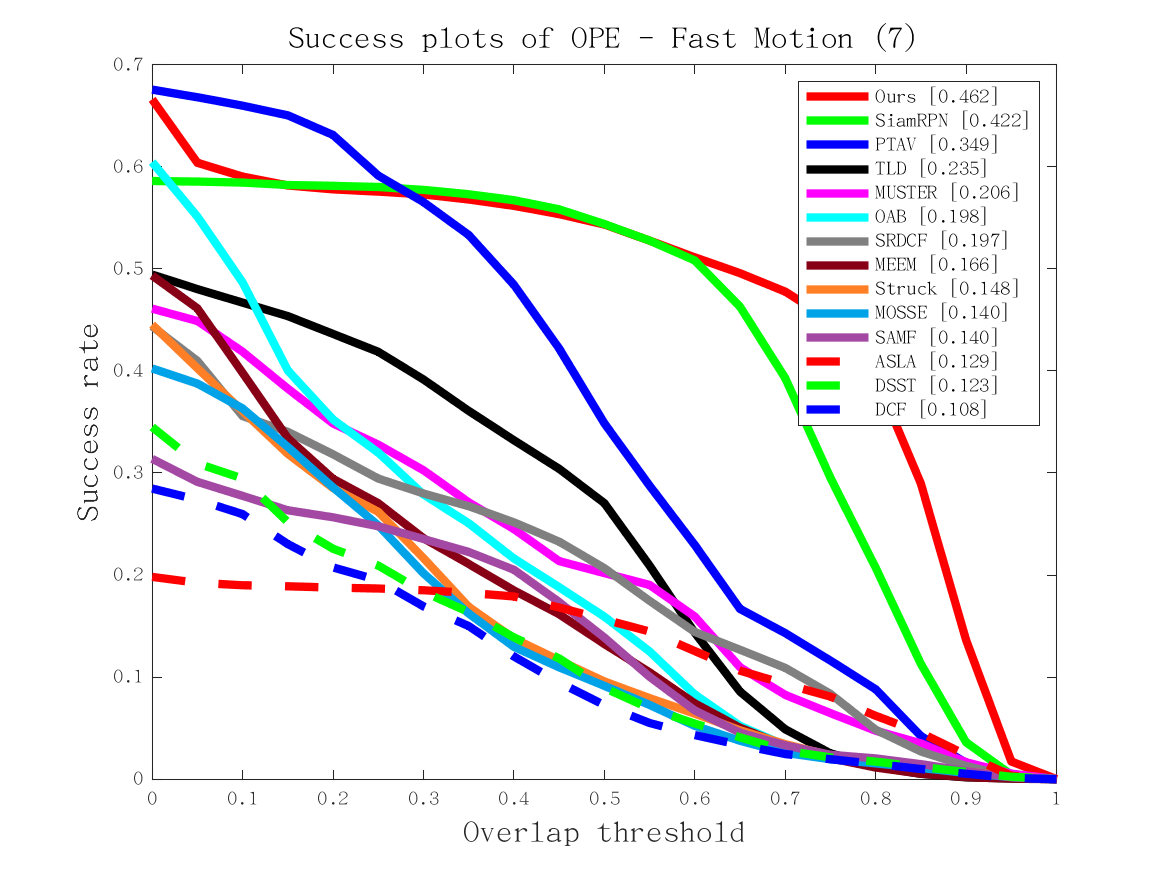
\includegraphics[width=0.48\textwidth]{Img/globally/UAV20L/FM_overlap_OPE_AUC.png}
	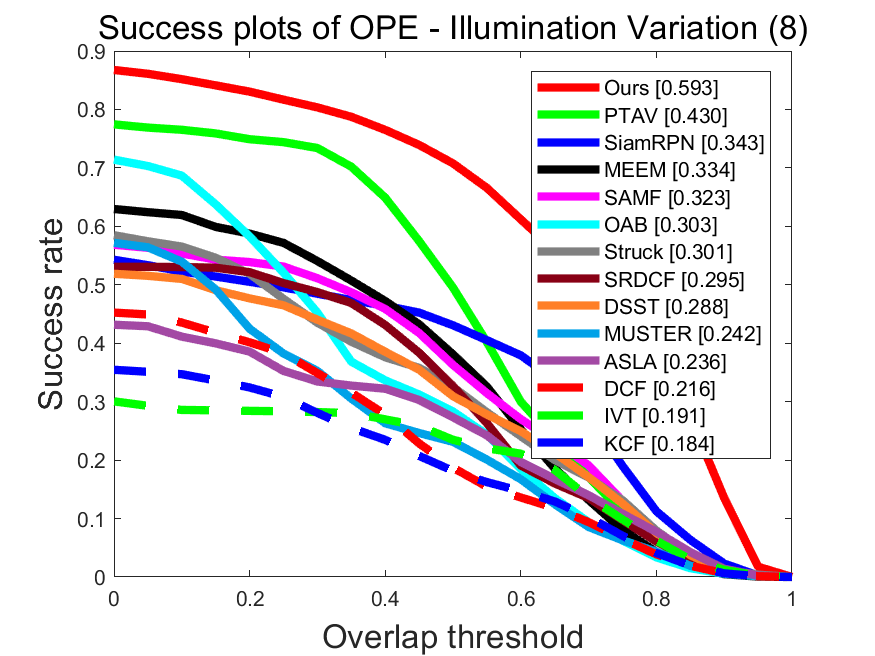
\includegraphics[width=0.48\textwidth]{Img/globally/UAV20L/IV_overlap_OPE_AUC.png}
	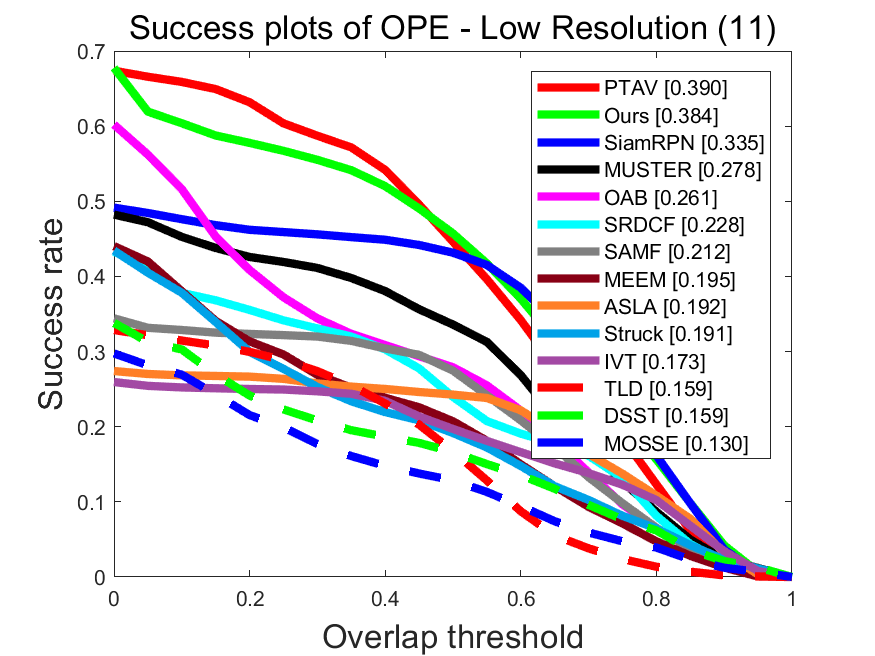
\includegraphics[width=0.48\textwidth]{Img/globally/UAV20L/LR_overlap_OPE_AUC.png}
	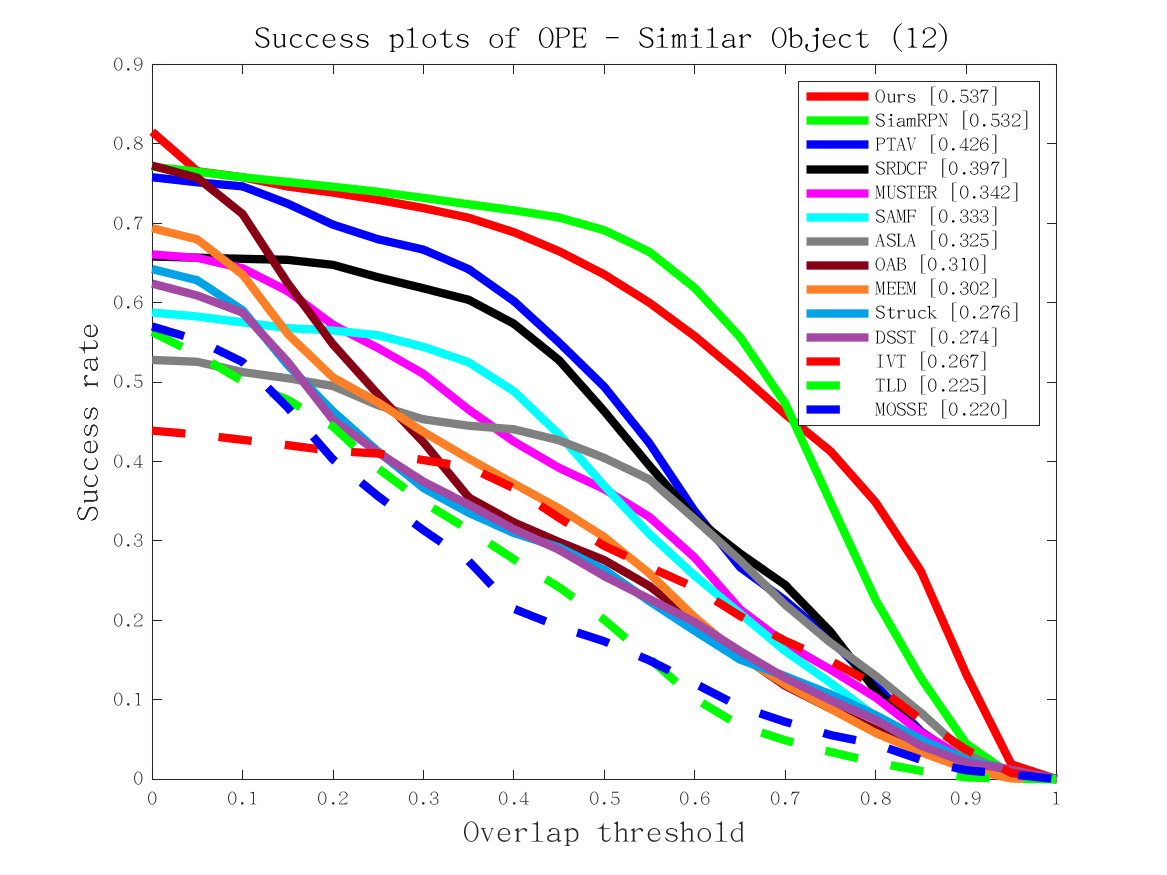
\includegraphics[width=0.48\textwidth]{Img/globally/UAV20L/SOB_overlap_OPE_AUC.png}
	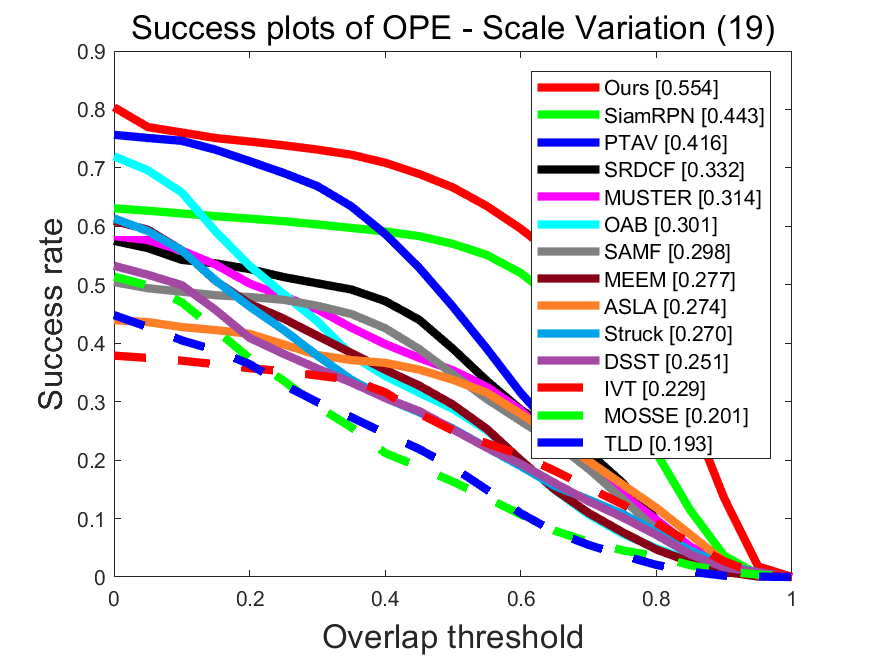
\includegraphics[width=0.48\textwidth]{Img/globally/UAV20L/SV_overlap_OPE_AUC.png}
	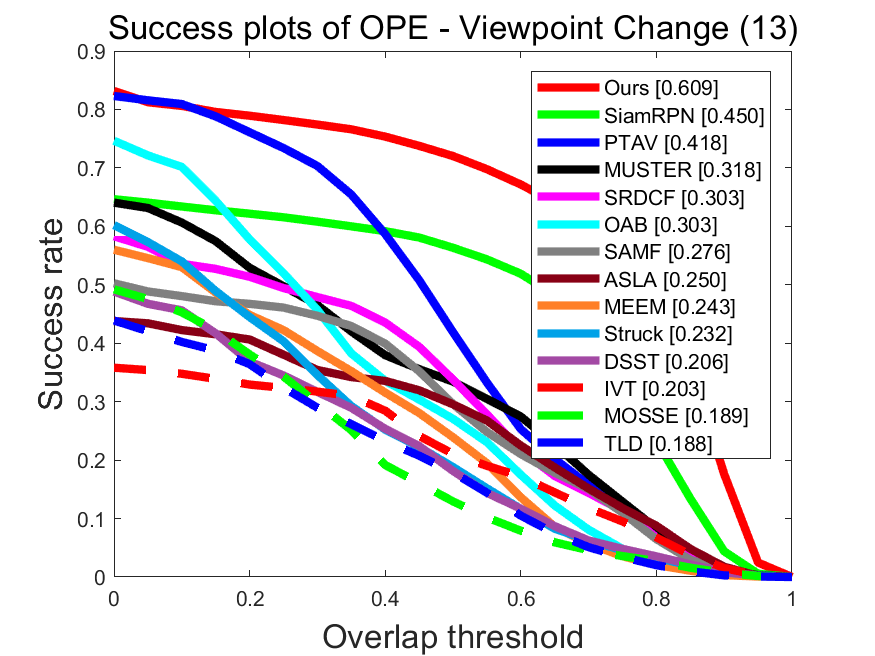
\includegraphics[width=0.48\textwidth]{Img/globally/UAV20L/VC_overlap_OPE_AUC.png}
\end{center}
   \caption{在 UAV20L 上成功绘制带有属性的图 2。在彩色显示屏上观看效果最佳。}
\label{fig:globally_uav20l_2}
\end{figure*}

\nopagebreak[3]
\begin{figure}[p!]
    \centering
    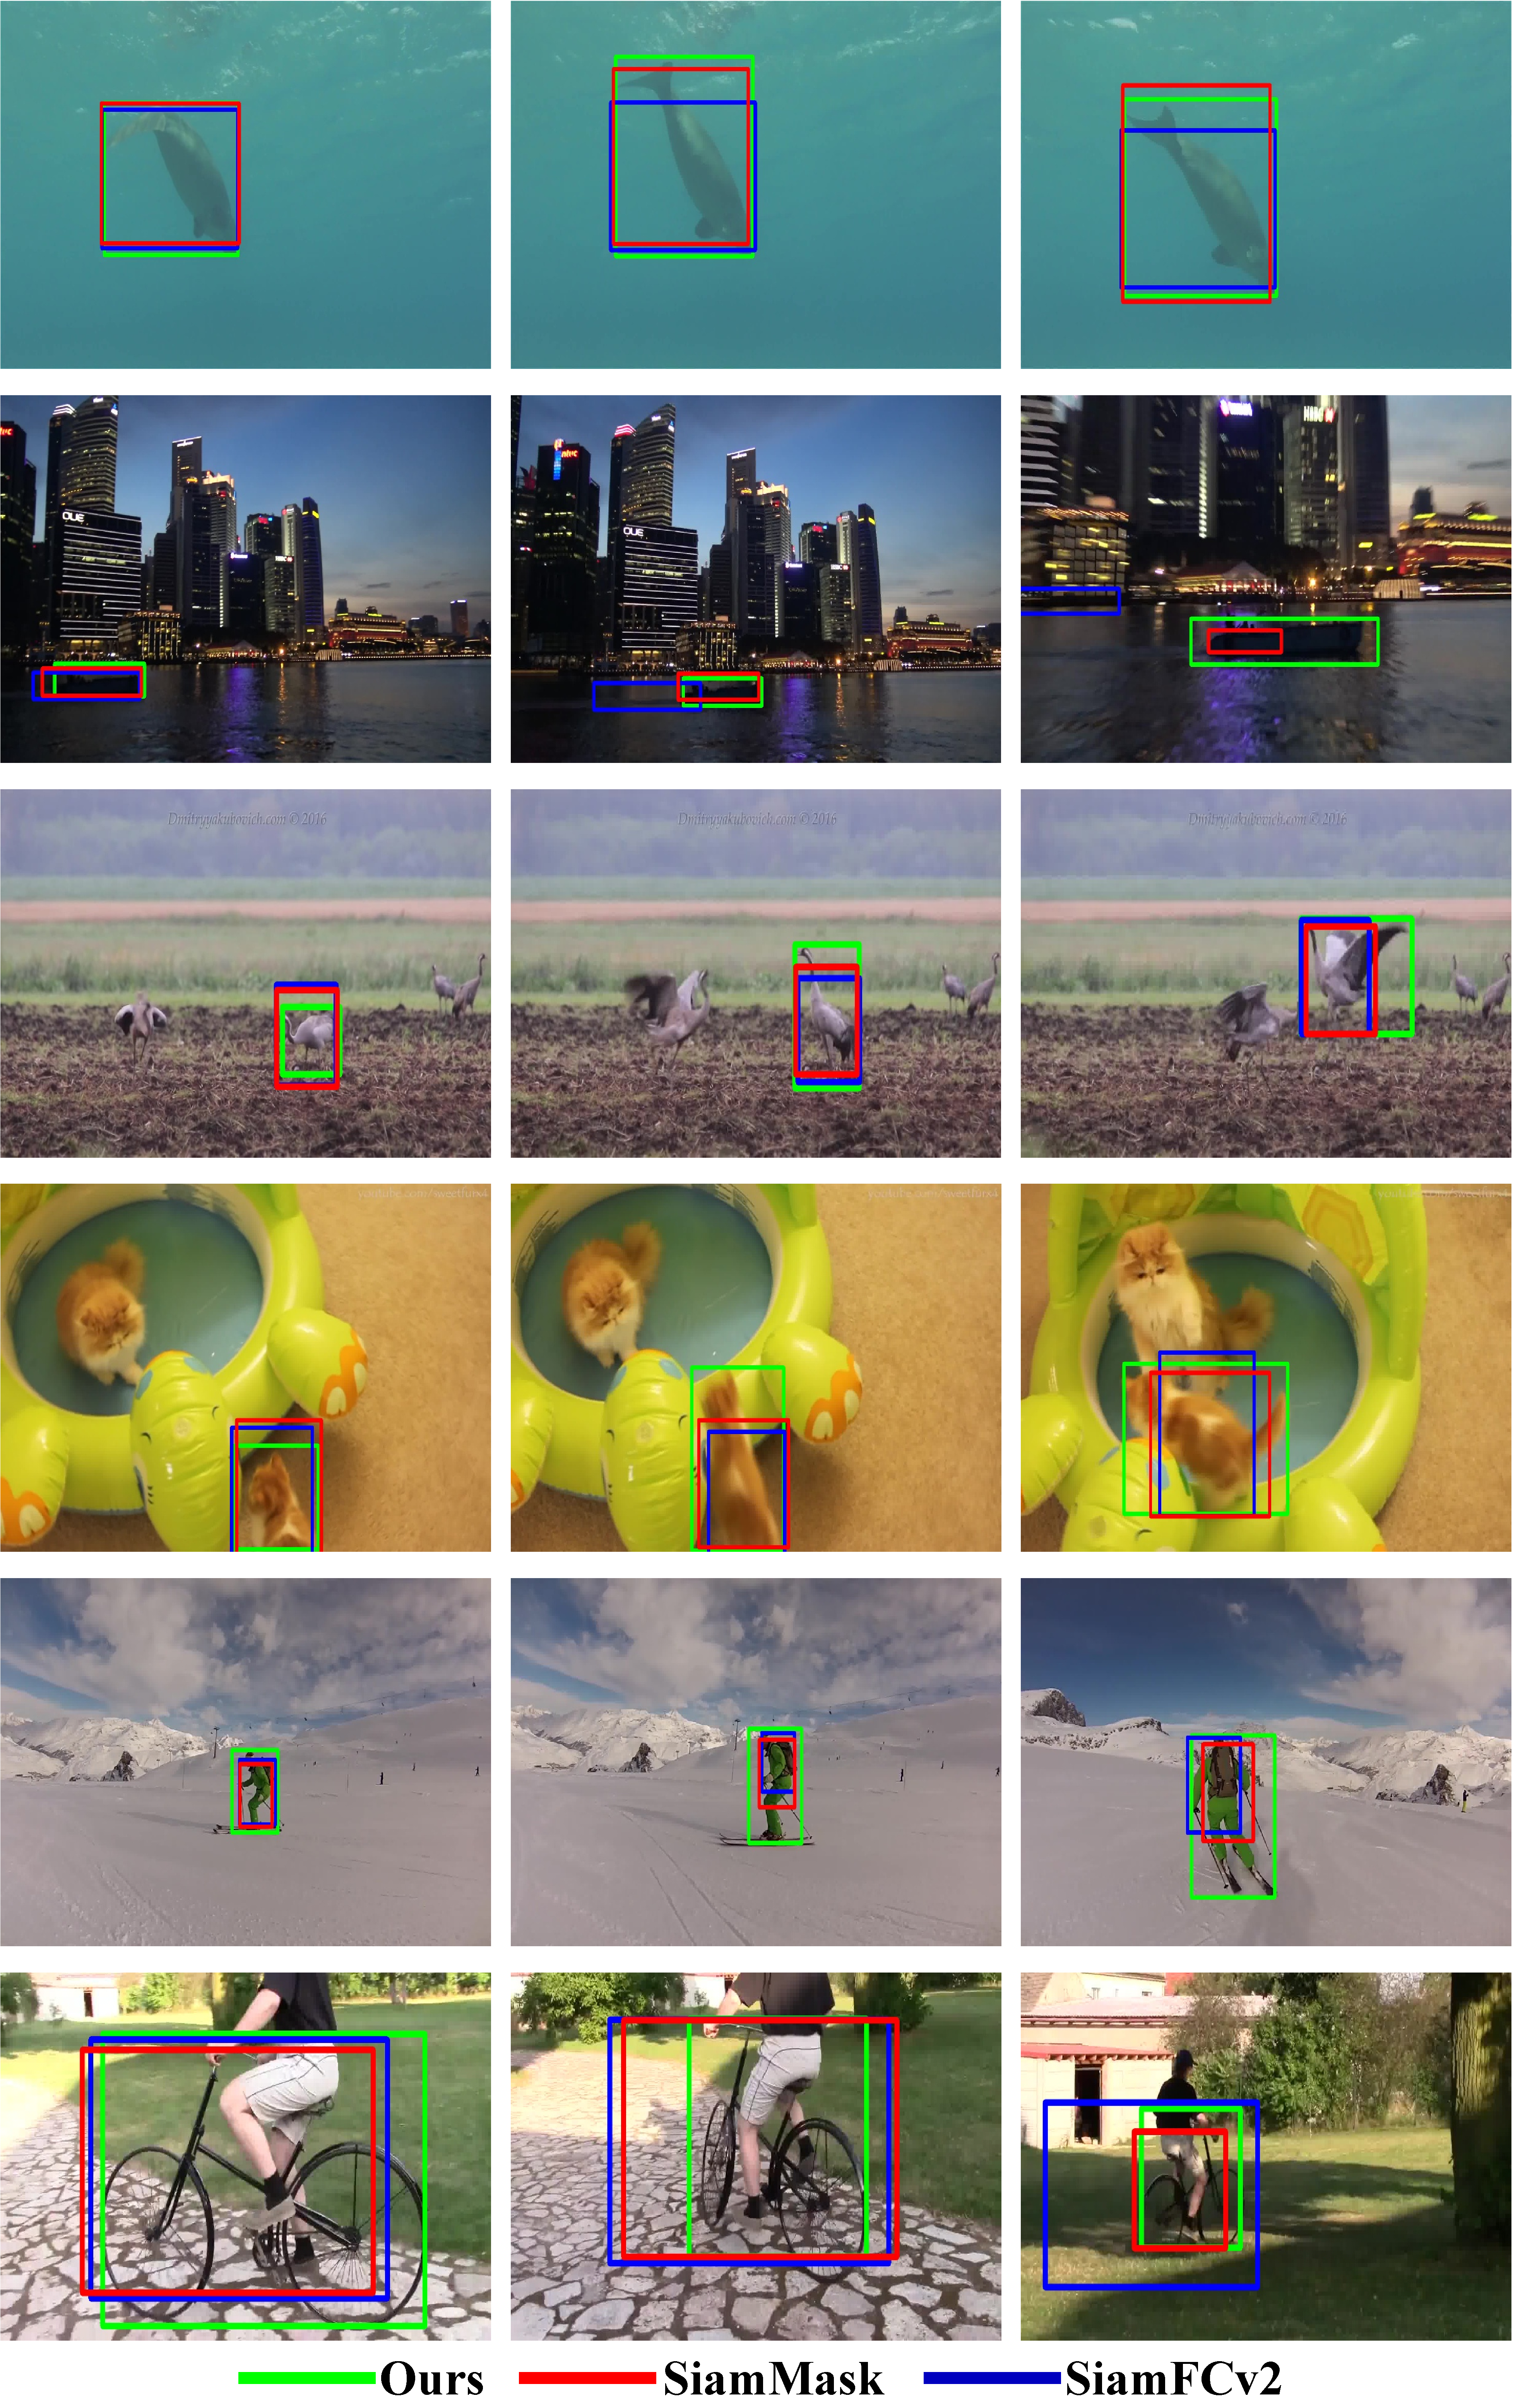
\includegraphics[width=0.9\textwidth]{Img/globally/visulization.pdf}
    \caption{本章提出的跟踪器与主流跟踪器 SiamMask \cite{Wang2018SiamMask} 和SiamFCv2\cite{SiamFC} 的比较。示例帧来自 GOT-10k \cite{GOT-10k} 测试集。}
    \label{fig:gloablly_vis}
\end{figure}
\nopagebreak[3]

\textbf{总体效果}
我们在 GOT-10k 测试集上将本章提出的方法与 8 个跟踪器(包括最新提出的跟踪器)进行了比较。
与列出的方法相比,我们的方法实现了 0.560 的 AO 得分(表 \ref{table:got})。
CSK 是基于 DCF 的典型跟踪器之一,它使用有效的循环矩阵理论导出闭式解,并使用使用几种类型的核进行训练和跟踪。相反,本章提出的跟踪器基于特征提取能力更强的卷积神经网络。因此,本章提出的跟踪器在 AO 得分方面远超 CSK,相对提升为 173.17%,这证明了卷积神经网络出色的特征表示能力以及本章提出的算法的有效性。
MDNet 具有多个分支,可学习共享层和特定域的层,其中不同的域对应不同的训练序列,每个分支负责二进制分类以识别每个域中的目标。相比之下,本章提出的跟踪器通过对目标模板和搜索区域的特征表示进行互相关操作来学习通用相似度特征图。与 MDNet 相比,本章提出的跟踪器的 AO 得分相对提升为 87.29%,这表明孪生架构和互相关运算在视频跟踪任务中的有效性。
SiamMask 是最新的跟踪器之一,它是一个孪生跟踪器,并可利用非常深的卷积神经网络进行提取特征。SiamMask 利用区域生成子网来预测目标的位置。
与 SiamMask \cite{Wang2018SiamMask} 相比,本章提出的两阶段跟踪器是基于全局感知机制设计的,可以减少跟踪过程中的累积误差,另外,轨迹预测模块可抑制近似物体的干扰并提高跟踪的鲁棒性。因此,本章提出的跟踪器在 AO 方面的性能要比 SiamMask 高出 22.00%,体现了所提出的两阶段跟踪框架和轨迹预测模块的有效性。

\textbf{按属性进行的性能分析}
GOT-10k 训练/验证数据集中的每个视频都带有多个属性,包括:目标可见率、运动速度、视频长度和按图像边界切割。为了分析跟踪器在不同属性下的性能,我们将跟踪器与两个最新的跟踪器(即 SiamFC  \cite{SiamFC} 和 SiamMask \cite{Wang2018SiamMask})在 GOT-10k 验证集上进行了比较。我们根据属性注释从验证集中收集四个子集:FM(快速运动)子集,OC(遮挡)子集,CU(图像边界切割)子集和 LO(长视频)子集。
FM 子集包括目标运动速度很快的视频。
OC 子集包括目标经常被遮挡的视频。
CU 子集包括目标经常被图像边界切割的视频。
LO 子集包括验证集中最长的 40 段视频。
表 \ref{table:attribute} 展示了跟踪算法的不同属性下的性能。
在 FM 子集上,本章提出的方法在 AO 方面的表现优于 SiamMask \cite{Wang2018SiamMask},相对提升为 21.48\%。
%This result suggests that our motion model is capable of modeling challenging motion patterns.
在 AO 方面,本章提出的算法在 OC 和 CU 子集上的性能分别比 SiamMask 高 18.42% 和 24.03%。
%This result suggests that our two-stage tracker based on ResNet50 is able to handle the appearance changes caused by heavy occlusion.
在 LO 子集上,与 SiamMask 相比,AO 得分的相对提升为 12.13%。结果表明,全局感知机制可以有效减少视频目标跟踪算法在跟踪长视频时的累积误差。

\subsection{对 UAV20L 数据集的评估}

UAV20L \cite{mueller2016benchmark} 是从低空鸟瞰视角捕获的航拍视频数据集。UAV20L 数据库专为长期跟踪而设计,包含 20 个视频,平均长度为 2934 帧。
遵循 OTB50 \cite{OTB} 的评估方法,我们使用精确度和成功率来评估 UAV20L 数据集上跟踪器的性能。精确度反映了指从预测边界框的中心点到真实边界框的中心点的距离。成功使用预测边界框与真实边界框的边框重叠计算得到。在图 \ref{fig:globally_uav20l} 中,不同跟踪器的性能比较通过精度图和成功图进行可视化。

我们将本章提出的方法与 13 个主流跟踪器进行了比较。图 \ref{fig:globally_uav20l} 清楚地表明,本章提出的算法在成功率和精确度得分方面均由于所提出的其他跟踪器。具体来说,在成功图中,我们的跟踪器获得的 AUC 得分为 0.557。与主流方法 PTAV \cite{fan2018parallel} 和 SiamRPN \cite{SiamRPN} 相比,本章提出的跟踪器的相对 AUC 提升分别为 31.7% 和 22.7%。在精度图中,本章所提算法的得分为 0.776。与 SiamRPN \cite{SiamRPN} 和 PTAV \cite{fan2018parallel} 相比,本章所提出的跟踪器的相对性能提升分别为 25.8\% 和 24.4\%。

此外,我们对 UAV20L 进行了基于属性的分析(参见图 \ref{fig:globally_uav20l_1} 和图 \ref{fig:globally_uav20l_2})。UAV20L 包含常见的视觉跟踪挑战,包括宽高比变化(aspect ration change,ARC)、背景混杂(background clutter,BC)、相机运动(camera motion,CM)、快速运动(fast motion,FM)、完全遮挡(Full Occlusion,FOC)、光照变化(illumination variation,IV)、低分辨率(low resolution,LR)、视线外(out-of-view,OV)、部分遮挡(partial occlusion,POC)、相似目标(similar object,SOB)、尺度变化(scale variation,SV)和视点改变(viewpoint change,VC)。
与所列出的方法相比,本章提出的方法在所有属性下均取得了最好的跟踪结果。
在文献 \cite{SiamRPN} 中,Li 等人提出了同时具有分类分支和回归分支的跟踪框架 SiamRPN。分类分支旨在在搜索图像中确定目标的位置,回归分支旨在优化目标的边框尺寸与长宽比。通过两个分支的合作,SiamRPN 具有较高的跟踪性能。因此,该算法在尺度变化、视点改变等属性上得分较高。尽管如此,SiamRPN 与本文提出的算法仍具有较大差距。比如在完全遮挡属性中,SiamRPN 的成功率仅为 0.192,而本章提出的算法成功率为 0.446。可能的原因是 SiamRPN 基于局部搜索机制进行跟踪,而本章提出的跟踪器采用了全局感知机制和轨迹预测模块,能够在目标再次出现在画面后及时进行继续跟踪。

\iffalse
In order to perform a more in-depth and detailed analysis of the performance of the trackers, we also report the results on challenging attributes in UAV20L. Fig. \ref{fig:uav20l_attr} lists the success plots of 14 different methods on 12 attributes: ARC (Aspect Ratio Change), BC (Background Clutter), CM (Camera Motion), FM (Fast Motion), FOC (Full Occlusion), IV (Illumination Variation), LR (LR Low Resolution), OV (Out-of-View), POC (Partial Occlusion), SOB (Similar Object), SV (Scale Variation) and VC (Viewpoint Change). We can observe that the AUC of the proposed algorithm perform better than other methods on most challenging attributes, which means our method is more robust than other approaches on various difficult situations.
\fi
\section{本章小结}
在本章中,我们提出了一种空间信息增强的视频目标跟踪算法,其中包括基于全局感知机制的两阶段跟踪框架和数据驱动的轨迹预测模块。全局感知机制允许跟踪组件减少跟踪过程中的累积误差。跟踪框架使用非常深的网络进行两阶段跟踪,使跟踪器提取的特征更具判别性。轨迹预测模块通过端到端训练,能够从大规模轨迹数据集中学习目标的运动模式。通过基于全局感知机制的两阶段跟踪框架和轨迹预测模块的协同工作,本章所提出的方法可实现较好的跟踪性能。